\documentclass{homework}
% \usepackage{lua-visual-debug}
% \usepackage[a4paper, total={6in, 8in}]{geometry}
\usepackage{graphicx}
\usepackage{float}
\usepackage{hyperref}
\usepackage{enumitem}

\title{Wireshark \#1}
\subject{CS341 Introduction to Computer Networks}
\studentid{20170058}
\name{Keonwoo Kim}
\date{\today}

\setstretch{1.0}

\begin{document}
\maketitle

\begin{figure}[H]
  \centering
  \hspace*{-0.2\textwidth}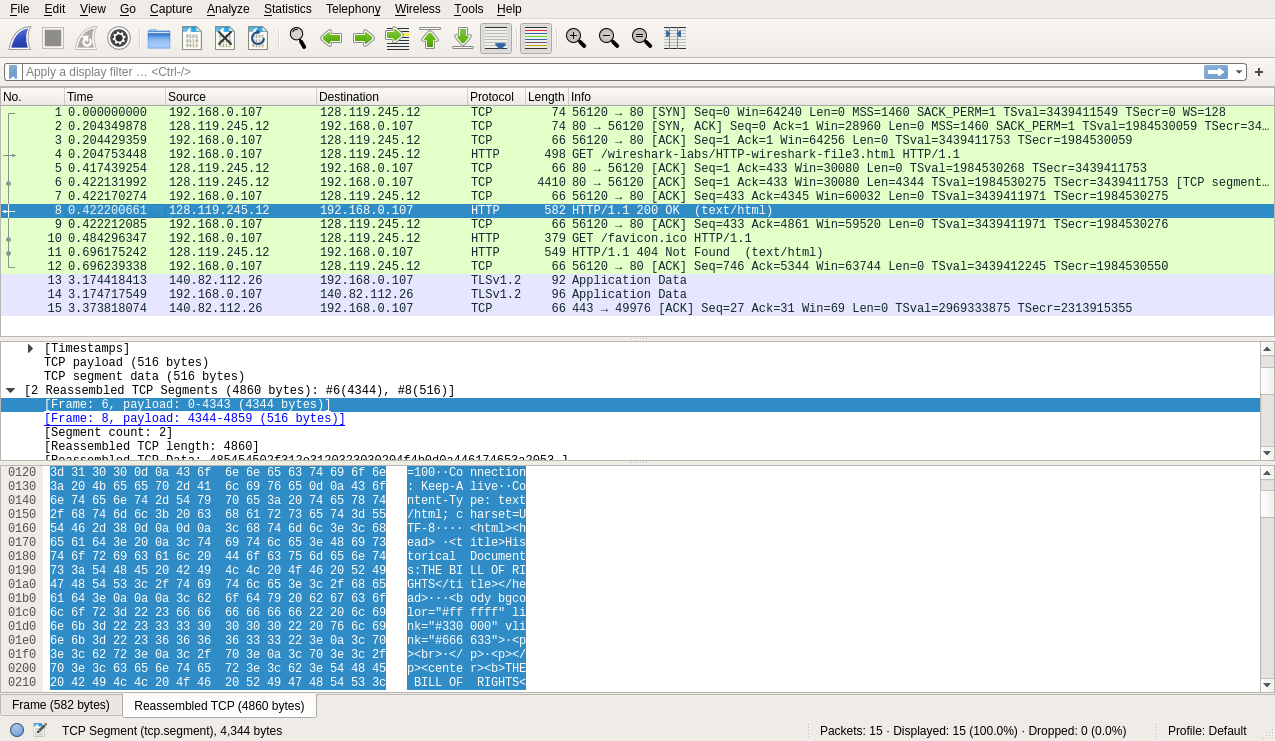
\includegraphics[width=1.4\textwidth]{file3-image}
  \caption{Sniffed packets while visiting \url{http://gaia.cs.umass.edu/wireshark-labs/HTTP-wireshark-file3.html}}
\end{figure}
\vspace*{2em}

\begin{enumerate}[label={(\arabic*)}]
  \item How many HTTP GET request messages were sent by your browser?
  
  \textsf{[Answer]} There were 2 HTTP GET requests sent by the browser: one for requesting \texttt{HTTP-wireshark-file3.html}, and the other for requesting \texttt{favicon.ico}.

  \item How many data-containing TCP segments were needed to carry the single HTTP response?
  
  \textsf{[Answer]} There were 2 TCP segments containing data for the html file, namely \#6 and \#8.

  \item What is the status code and phrase associated with the response to the HTTP GET request?
  
  \textsf{[Answer]} Req \#4, resp \#8: the status code was \texttt{200}, and the status text was \texttt{OK}. \\
  Req \#10, resp \#11: the status code was \texttt{404}, and the status text was \texttt{Not found}.

  \item Which packet number in the trace contains the GET message for the Bill \underline{of} Rights?
  
  \textsf{[Answer]} \#4

  \newpage

  \begin{figure}[H]
    \centering
    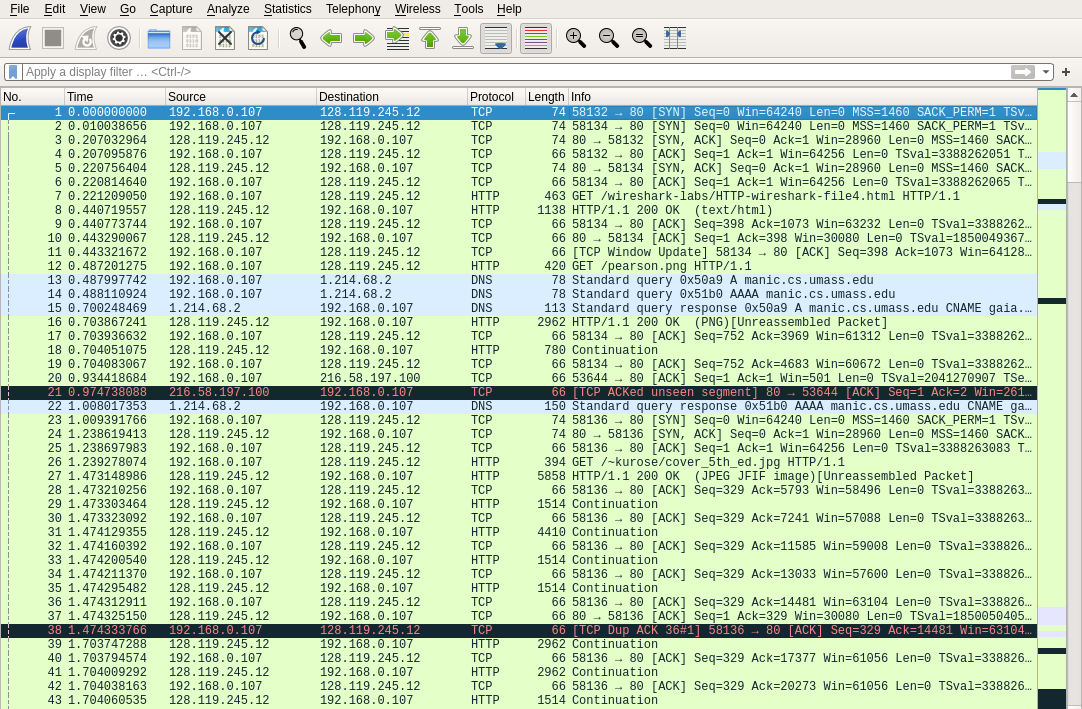
\includegraphics[width=\textwidth]{file4-image-0}
    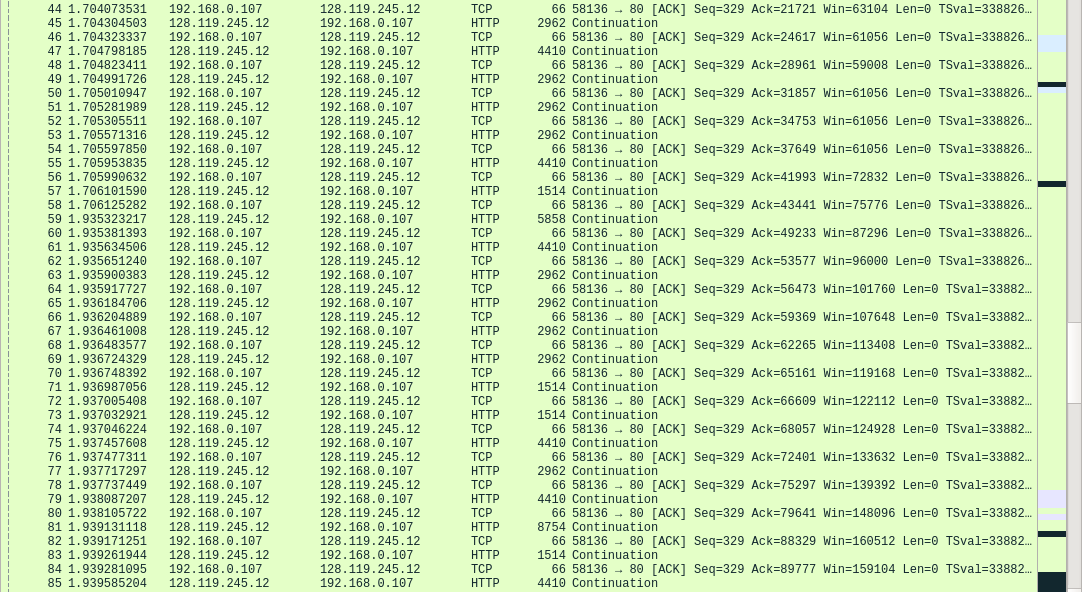
\includegraphics[width=\textwidth]{file4-image-1}
    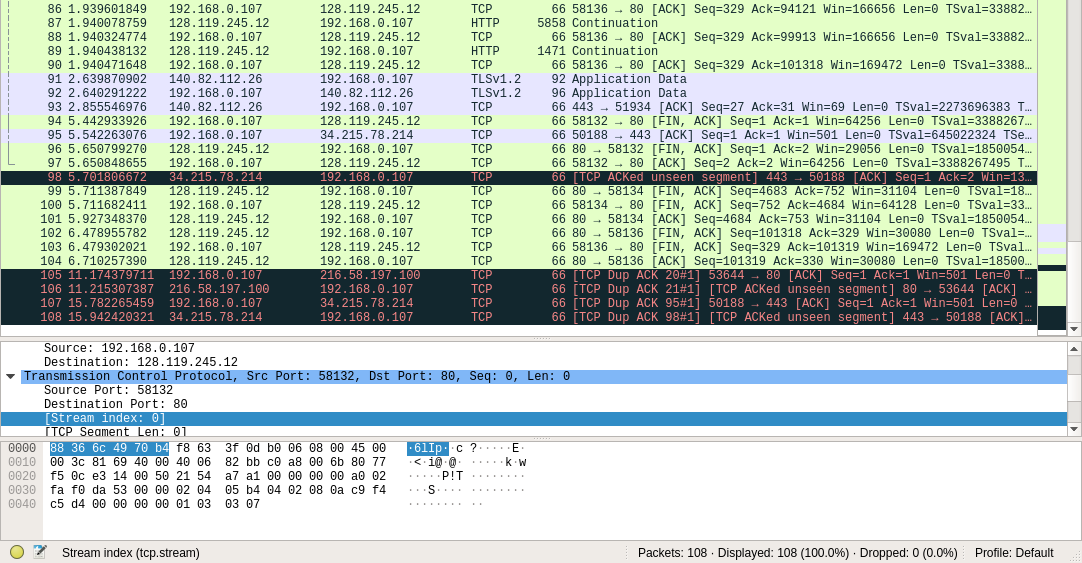
\includegraphics[width=\textwidth]{file4-image-2}
    \caption{Sniffed packets while visiting \url{http://gaia.cs.umass.edu/wireshark-labs/HTTP-wireshark-file4.html}}
  \end{figure}

  \begin{figure}[H]
    \centering
    \hspace*{-0.1\textwidth}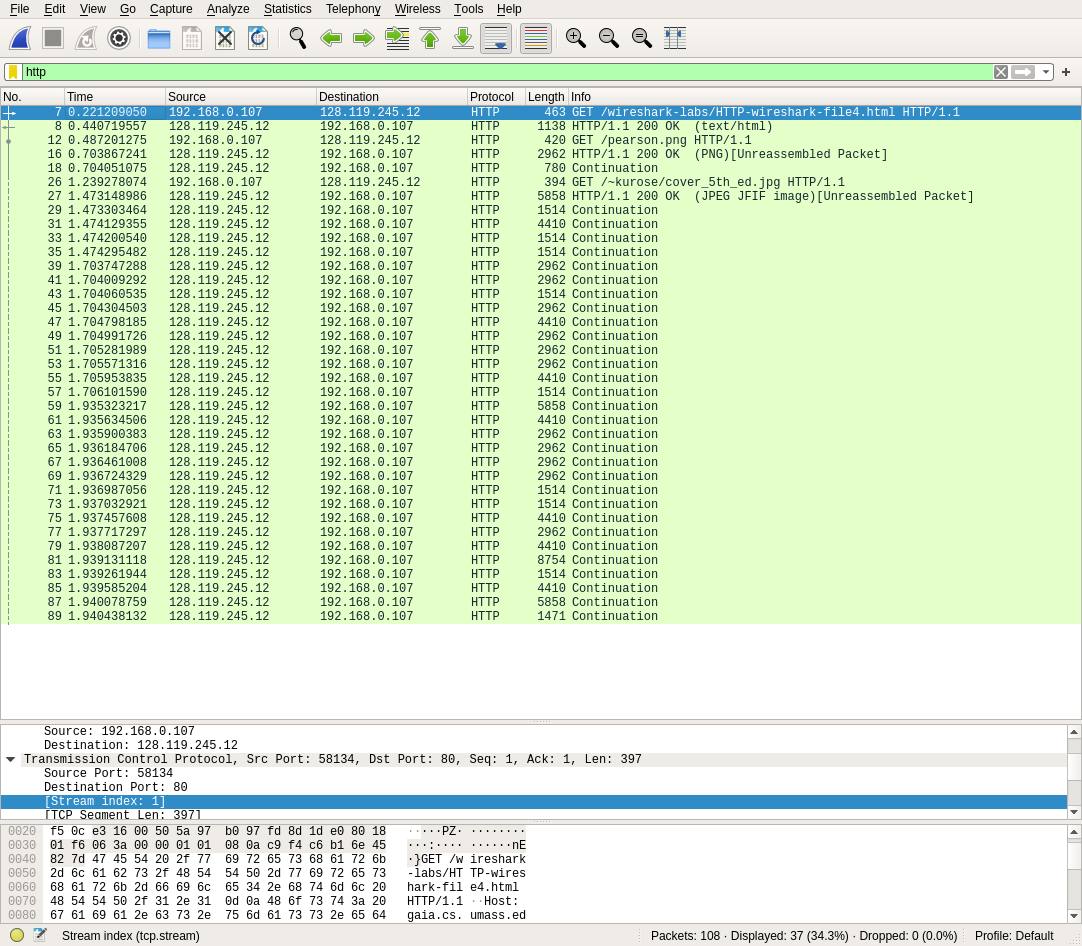
\includegraphics[width=1.2\textwidth]{file4-image-http-only}
    \caption{Sniffed packets while visiting \url{http://gaia.cs.umass.edu/wireshark-labs/HTTP-wireshark-file4.html}, filtering the http responses only}
  \end{figure}

  \item How many HTTP GET request messages were sent by your browser? To which Internet addresses were these GET requests sent?

  \textsf{[Answer]} There are 3 HTTP GET request messages were sent by the browser: for requesting \texttt{HTTP-wireshark-file4.html}, \texttt{pearson.png}, and \texttt{cover\_5th\_ed.jpg}. All 3 requests are sent to the IP address \texttt{128.119.245.12}.
  
  The reason why the browser did not try to download the favicon, which is a different behavior from the result of (1), is because of the cache feature of the browser.
  
  \item Can you tell whether your browser downloaded the two images serially, or whether they were downloaded from the two web sites in parallel? Explain.
  
  \textsf{[Answer]} They were downloaded serially. We can identify which requests and continuations correspond to which file streams via seeing the stream index. The HTTP response \#16 and \texttt{Continuation} \#18 were indexed by the stream index \texttt{1}, and the HTTP response \#27 and the \texttt{Continuation}s after \#18, which are \#29, \#31, \ldots, \#89, were indexed by the stream index 3. Thus, we notice that the browser started to download \texttt{cover\_5th\_ed.jpg} from \texttt{/\string~kurose/cover\_5th\_ed.jpg} after downloading \texttt{pearson.png} completely. Hence, the download of two files was done serially.
\end{enumerate}

\end{document}